
\section*{Results}


In order to keep this article  succinct, in the following we only report a subset of the results. The remaining results (which show similar trends to those reported here) are made available in the appendix material  for completeness.  \textit{All data and code will be shared on GitHub upon acceptance.}
%\url{https://sites.google.com/view/understandabilityontheweb/}.

\subsection*{Evaluation of understandability estimators}
\label{sec:beyond_readability}


\begin{table*}[t]
\centering \caption{Methods with the highest correlation per category for CLEF 2015 eHealth
collection. Bold is used to highlight the best result of each group.}
\label{tab:top_corr_metrics} \resizebox{.55\textwidth}{!}{ %%%%
\begin{tabular}{lccccc}
\toprule 
\textbf{Cat.}  & \textbf{Method}  & \textbf{Preproc.}  & \textbf{Pears.} & \textbf{Spear.}  & \textbf{Kend.} \tabularnewline
\midrule 
\textbf{RF} & SMOG Index & Jst NFP  & \textbf{.438} & \textbf{.388} & \textbf{.286}\tabularnewline
\midrule 
\multirow{2}{*}{\textbf{CRF}}  & Avg. Num. of Polysyl. Words per Word  & Jst FP  & \textbf{.429} & .364 & .268\tabularnewline
 & Avg. N. of Polysyl. Words per Sentence  & Jst NFP  & .192 & \textbf{.388} & \textbf{.286}\tabularnewline
\midrule 
\multirow{2}{*}{\textbf{GMV}}  & Avg. N. Medical Prefixes per Word  & \multirow{2}{*}{Naive FP}  & \textbf{.314} & .312 & .229 \tabularnewline
 & Number of Medical Prefixes  &  & .131 & \textbf{.368} & \textbf{.272} \tabularnewline
\midrule 
\textbf{CMV} & CHV Mean Score for all Concepts & Naive FP & \textbf{.371} & \textbf{.314} & \textbf{.228}\tabularnewline
\midrule 
\textbf{EMV}  & Number of MeSH Concepts & Naive FP  & \textbf{.227} & \textbf{.249} & \textbf{.178} \tabularnewline
\midrule 
\multirow{2}{*}{\textbf{NLF}}  & N. of words not found in Aspell Dict.  & Jst NFP  & \textbf{.351}  & .276  & .203 \tabularnewline
 & Number of Pronouns per Word  & Naive FP  & .271  & \textbf{.441}  & \textbf{.325} \tabularnewline
\midrule 
\textbf{HF} & Number of P Tags & None & \textbf{.219} & \textbf{.196}  & \textbf{.142} \tabularnewline
\midrule 
\multirow{2}{*}{\textbf{WFF}}  & Mean Rank Medical Reddit - Includes OV  & Jst NFP  & \textbf{.435}  & .277  & .197 \tabularnewline
 & 25th percentil Pubmed  & Jst NFP  & .330  & \textbf{.347}  & \textbf{.256} \tabularnewline
\midrule 
\multirow{2}{*}{\textbf{MLR}}  & \multirow{2}{*}{eXtreme Gradient Boosting (XGB) Regressor}  & Boi NFP  & \textbf{.602}  & .394  & .287 \tabularnewline
 &  & Jst FP  & .565  & \textbf{.438}  & \textbf{.324} \tabularnewline
\midrule 
\textbf{MLC}  & Multinomial Naive Bayes  & Naive FP  & \textbf{.573}  & \textbf{.477}  & \textbf{.416} \tabularnewline
\bottomrule
\end{tabular}} %%%%% ---- 
\end{table*}

\begin{table*}[t]
\centering \caption{Methods with the highest correlation per category for CLEF 2016 eHealth
collection. Bold is used to highlight the best result of each group.}
\label{tab:top_corr_metrics2016} \resizebox{.55\textwidth}{!}{ %%%%
\begin{tabular}{lccccc}
\toprule 
\textbf{Cat.}  & \textbf{Method}  & \textbf{Preproc.}  & \textbf{Pears.}  & \textbf{Spear.}  & \textbf{Kend.}\tabularnewline
\midrule 
\multirow{2}{*}{\textbf{RF}}  & \multirow{2}{*}{Dale-Chall Index }  & Jst FP  & \textbf{.439}  & .381  & .264\tabularnewline
 &  & Boi FP  & .437  & \textbf{.382}  & \textbf{.264}\tabularnewline
\midrule 
\textbf{CRF} & Avg. Difficult Words Per Word & Boi FP  & \textbf{.431}  & \textbf{.379}  & \textbf{.262}\tabularnewline
\midrule 
\multirow{2}{*}{\textbf{GMV}}  & Avg. Prefixes per Sentence  & Jst FP  & \textbf{.263}  & .242  & .164\tabularnewline
 & ICD Concepts Per Sentence  & Jst NFP  & .014  & \textbf{.253}  & \textbf{.172}\tabularnewline
\midrule 
\multirow{2}{*}{\textbf{CMV}}  & CHV Mean Score for all Concepts  & Jst FP  & \textbf{.329}  & .313  & .216\tabularnewline
 & CHV Mean Score for all Concepts  & Boi FP  & .329  & \textbf{.325}  & \textbf{.224}\tabularnewline
\midrule 
\multirow{2}{*}{\textbf{EMV}}  & Number of MeSH Concepts  & \multirow{2}{*}{Boi NFP }  & \textbf{.201}  & .166  & .113\tabularnewline
 & Number of MeSH Disease Concepts  &  & .179  & \textbf{.192}  & \textbf{.132}\tabularnewline
\midrule 
\multirow{2}{*}{\textbf{NLF}}  & Avg. Stopword Per Word  & \multirow{2}{*}{Boi FP }  & \textbf{.344}  & .312  & .213\tabularnewline
 & Number of Pronouns  &  & .341  & \textbf{.364}  & \textbf{.252}\tabularnewline
\midrule 
\multirow{2}{*}{\textbf{HF}}  & Number of Lists  & \multirow{2}{*}{None}  & \textbf{.114}  & .021  & .015\tabularnewline
 & Number of P Tags  &  & .110  & \textbf{.123}  & \textbf{.084}\tabularnewline
\midrule 
\multirow{2}{*}{\textbf{WFF}}  & Mean Rank Medical Reddit  & Boi NFP  & \textbf{.387}  & .312  & .214\tabularnewline
 & 50th percentil Medical Reddit  & Jst NFP  & .351  & \textbf{.315}  & \textbf{.216}\tabularnewline
\midrule 
\multirow{2}{*}{\textbf{MLR}}  & eXtreme Gradient Boosting (XGB) Regressor  & Jst NFP  & \textbf{.454}  & \textbf{.373}  & .258\tabularnewline
 & Random Forest Regressor  & Boi NFP  & .389  & .355  & \textbf{.264}\tabularnewline
\midrule 
\textbf{MLC}  & Multinomial Naive Bayes  & Jst FP  & \textbf{.461}  & \textbf{.391}  & \textbf{.318}\tabularnewline
\bottomrule
\end{tabular}} %%%%% ---- 
\end{table*}


Using the CLEF eHealth 2015 and 2016 collections, we studied the correlations of methods to estimate Web page understandability (Table~\ref{tab:doc_features}), compared with human assessments. For each category of understandability estimation, Tables~\ref{tab:top_corr_metrics2015} and \ref{tab:top_corr_metrics2016} report the methods with highest Pearson, Spearman or Kendall correlations for CLEF eHealth 2015 and 2016 collections, respectively. For each method, we used the best preprocessing settings; a study of the impact of preprocessing is reported in the next subsection.

Overall, Spearman and Kendall correlations obtained similar results (in terms of which methods exhibited the highest correlations): this was expected as, unlike Pearson, they are both rank-based correlations.

For traditional readability measures, SMOG had the highest correlations for CLEF 2015 and DCI for CLEF 2016, regardless of correlation measure. These results resonate with those obtained for the category of raw components of readability formulas. 
In fact, the polysyllable words measure, which is the main feature used in SMOG, had the highest correlation for CLEF 2015 among methods in this category. Similarly, the number of difficult words, which is the main feature used in DCI, had the highest correlation for CLEF 2016 among methods in this category.

When examining the expert vocabulary category, we found that the number of MeSH concepts obtained the highest correlations with human assessments; however, its correlations were substantially lower than those achieved by the best method from the consumer medical vocabularies category, i.e. the scores of CHV concepts. For the natural language category, we found that the number of pronouns, the number of stop words and the number of out of vocabulary words had the highest correlations -- and these were even higher than those obtained with MeSH and CHV based methods. In turn, the methods that obtained the highest correlations among the HTML category (counts of P tags and list tags) exhibited overall the lowest correlations compared to methods in the other categories. P tags are used to create paragraphs in a Web page, being thus a rough proxy for text length. 
Among methods in the word frequency category, the use of Medical Reddit (but also of PubMed) showed the highest correlations, and these were comparable to those obtained by the readability formulas. 

Finally, regressors and classifiers exhibited the highest correlations amongst all methods: in this  category, the  eXtreme Gradient Boosting (XGB) regressor and the multinomial Naive Bayes best correlated with human assessments. 

\subsection*{Evaluation of Preprocessing Pipelines and Heuristics}
\label{sec:which_preprocessing}

Results from experiments with different preprocessing pipelines and heuristics are shown in Figure~\ref{fig:boxplot_corr_docs} (top: CLEF 2015; bottom: CLEF 2016). 
For each category of methods and combination of preprocessing and heuristics, we report their variability in terms of Spearman rank correlation with human assessments. Results for Pearson and Kendall correlations are reported in the appendix, but showed similar trends. 
We further report the summary results across all understandability assessment methods and sentence-ending heuristics for each of the preprocessing pipelines. 
Finally, we also report the inter-assessor correlation (last box) when multiple assessors provided judgements about the understandability of Web pages. % (details about this data in Section~\ref{sec:data}). 
This provides an indication of the range of variability and subjectiveness when assessing understandability, along with the highest correlation we measured between human assessors. 

\begin{figure*}[h!]
   \centering
   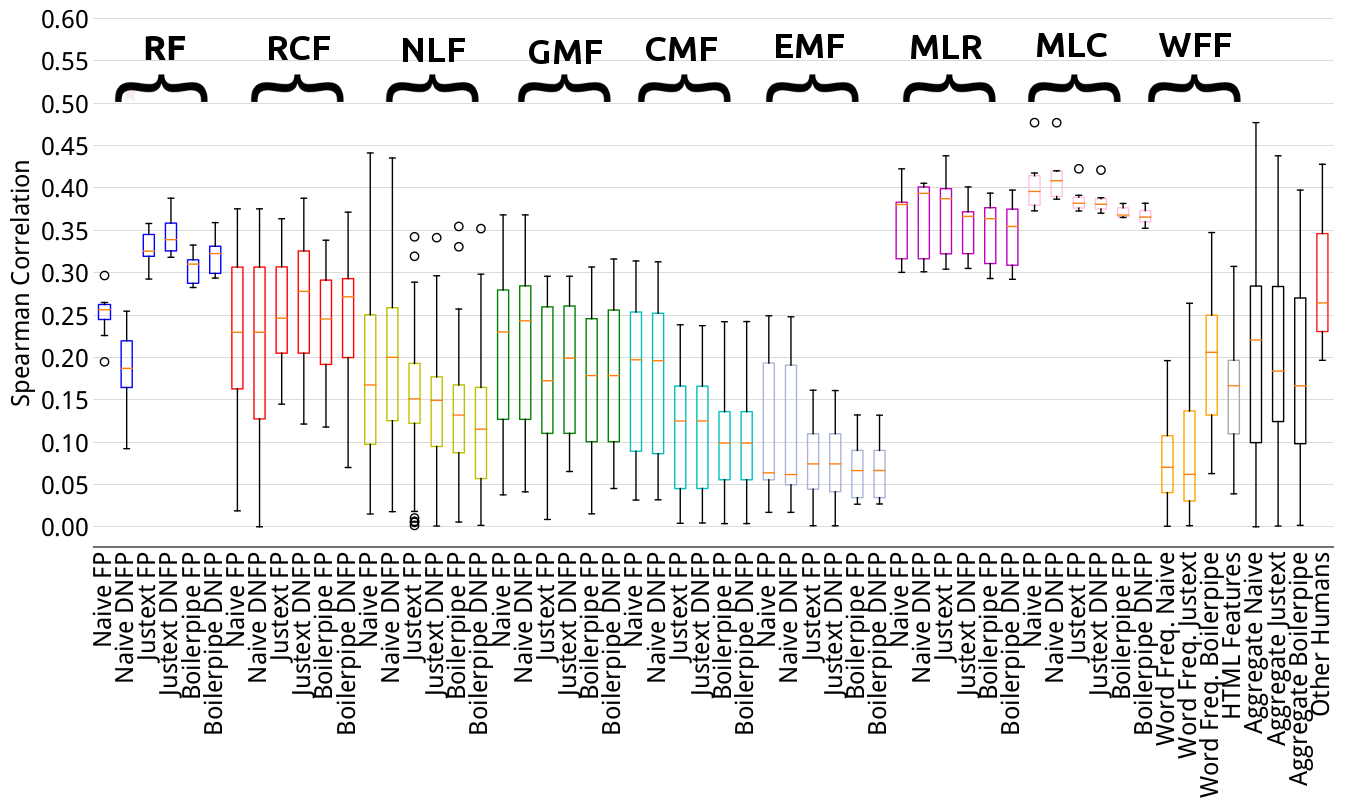
\includegraphics[width=0.85\textwidth]{graphics/box_spearman15_raw_values_joao}\vspace{-7pt}
      \includegraphics[width=0.85\textwidth]{graphics/box_spearman16_raw_values}
    \caption{Correlations between understandability estimators and human assessments for CLEF 2015 (top) and 2016 (bottom). For example, the first boxplot on the top represents the distribution of Spearman correlations with human assessments across all features in the category Readability Features (Table~\ref{tab:doc_features}), obtained with the Naive \textit{ForcePeriod} preprocessing, for CLEF 2015. Each box extends from the lower to the upper quartile values, with the red marker representing the median value for that category. Whiskers show the range of the data in each category and circles represent values considered outliers for the category (e.g., Spearman correlation for SMOG index was 0.296 and for ARI was 0.194: these were outliers for that category).} 
   \label{fig:boxplot_corr_docs}
   \vspace{-10pt}
\end{figure*}

We first examined the correlations between human assessments and readability formulas. We found that the \textit{Naive} preprocessing resulted in the lowest correlations, regardless of readability formula and heuristic (although \textit{DoNotForcePeriod} performed better than \textit{ForcePeriod}). Using Justext or Boilerplate resulted in higher correlations with human understandability assessments, and the \textit{ForcePeriod} heuristic was shown to be better than \textit{DoNotForcePeriod}. These results confirm the speculations of Palotti et al.~\cite{palotti15}: they found these settings to produce lower variances in understandability estimations and thus hypothesised that they were better suited to the task.

Overall, among readability formulas, the best results (highest correlations) were obtained by SMOG and DCI (see also Tables~\ref{tab:top_corr_metrics2015} and \ref{tab:top_corr_metrics2016}). Although no single setting outperformed the others in both collections, we found that the use of CLI and FRE with \textit{Justext} provided the most stable results across the collections, with correlations as high as the best ones in both collections.
These results confirmed the advice put forward by Palotti et al.~\cite{palotti15}, i.e. in general, if using readability measures, then CLI is to be preferred, along with an appropriate HTML extraction pipeline, regardless of the heuristic for sentence ending. We provide detailed plots to compare our results with Palotti's in the appendix.

When considering methods beyond those based on readability formulas, we found that the highest correlations were achieved by the regressors (MLR) and classifiers (MLC), independently of the preprocessing method used. There is little difference in terms of effectiveness of methods in these categories, with the exception of regressors on CLEF 2015 that exhibited not negligible variances: while for the Neural Network Regressor the Pearson correlation was 0.44, for the Support Vector Regressor it was only 0.30.

A common trend when comparing preprocessing pipelines is that the Naive pipeline provided the weakest correlations with human assessments for CLEF 2016, regardless of estimation methods and heuristics. This result, however, was not confirmed for CLEF 2015, where the Naive preprocessing negatively influenced correlations for the readability formula category (RF), but not for other categories, although it was generally associated with larger variances for the correlation coefficients.


\subsection*{Evaluation of Understandability Retrieval}
\label{sec:results}


%\begin{table}
\caption{Reports on the experiments with 4 base runs: the top 3 runs of CLEF eHealth 2017 and a plain baseline run. The second (indices 5-8) and third (indices 9-12) parts shows results of a RegressorTree based on top features from Table X. The forth part of this table shows results when reranking top 20 results based on Dale-Chall Index. Finally, we combine selected runs with reciprocal rank fusion in the last part of this table. Results shows that regression on top 15 improves
    understandability to the detriment of topical relevance. Regression on top 20 it is even more agreessive. Dale Chall presents the same logic, but understandability gains are smaller compared to regressor results. Finally, the combination with rrf yields the best $F_ru$ scores. I still need to compute if we get statistically significant improvements or not.}
\label{tab:experiments}
\begin{tabular}{c|c|c|ccc|cc|c|ccc}
\toprule 
Index & Rerank & Run & P\_r@10 & P\_u@10 & F\_ru & RBP & uRBP & Unj@10 & Pr@10 & Pu@10 & F\_ru{*}\tabularnewline
\midrule 
1 & \multirow{4}{*}{No Rerank} & BM25 Q.E. & 31.43 & 49.70 & 38.51 & 29.05 & 10.40 & 0.02 & 31.70 & 50.83 & 39.05\tabularnewline
2 &  & GUIR & 29.67 & 50.97 & 37.50 & 28.11 & 9.98 & 0.01 & 30.20 & 51.80 & 38.16\tabularnewline
3 &  & ECNU & 29.33 & 49.27 & 36.77 & 27.70 & 10.14 & 0.01 & 29.50 & 49.87 & 37.07\tabularnewline
4 &  & Plain BM25 & 26.47 & 46.33 & 33.69 & 25.28 & 9.22 & 0.06 & 27.63 & 48.93 & 35.32\tabularnewline
\midrule
5 & \multirow{4}{*}{Regress Top 15} & Based on Run 1 & 27.87 & 49.40 & 35.63 & 26.38 & 6.51 & 0.01 & 28.10 & 49.60 & 35.88\tabularnewline
6 &  & Based on Run 2 & 27.27 & 48.57 & 34.93 & 25.95 & 6.56 & 0.01 & 27.30 & 48.60 & 34.96\tabularnewline
7 &  & Based on Run 3  & 26.60 & 50.10 & 34.75 & 25.08 & 6.23 & 0.00 & 26.67 & 50.10 & 34.81\tabularnewline
8 &  & Based on Run 4 & 23.73 & 50.87 & 32.37 & 22.86 & 5.19 & 0.09 & 24.97 & 52.67 & 33.87\tabularnewline
\midrule 
9 & \multirow{4}{*}{Regress. Top 20} & Based on Run 1 & 27.70 & \textbf{52.13} & 36.18 & 26.10 & 5.95 & 0.02 & 28.17 & 52.53 & 36.67\tabularnewline
10 &  & Based on Run 2 & 26.70 & \textbf{53.10} & 35.53 & 25.44 & 5.81 & 0.01 & 26.83 & 53.33 & 35.70\tabularnewline
11 &  & Based on Run 3  & 26.17 & \textbf{52.67} & 34.96 & 24.88 & 5.59 & 0.02 & 26.43 & 53.17 & 35.31\tabularnewline
12 &  & Based on Run 4 & 23.30 & \textbf{51.43} & 32.07 & 22.53 & 4.51 & 0.12 & 25.10 & 55.20 & 34.51\tabularnewline
\midrule 
13 & \multirow{4}{*}{Dale-Chall top 20} & Based on Run 1 & 29.63 & 49.93 & 37.19 & 26.45 & 8.58 & 0.02 & 29.87 & 50.37 & 37.50\tabularnewline
14 &  & Based on Run 2 & 28.37 & 51.10 & 36.48 & 25.01 & 8.05 & 0.01 & 28.60 & 51.40 & 36.75\tabularnewline
15 &  & Based on Run 3  & 27.70 & 50.80 & 35.85 & 24.54 & 7.96 & 0.02 & 28.03 & 51.47 & 36.30\tabularnewline
16 &  & Based on Run 4 & 24.13 & 49.97 & 32.55 & 21.28 & 6.68 & 0.10 & 26.17 & 53.17 & 35.07\tabularnewline
\midrule
17 & \multirow{4}{*}{Reciprocal Rank Fusion} & Runs 1 and 9 & 30.70 & 52.37 & \textbf{38.71} & 27.93 & 7.63 & 0.02 & 31.10 & 53.30 & 39.28\tabularnewline
18 &  & Runs 2 and 10 & 30.67 & 51.90 & \textbf{38.55} & 28.34 & 8.14 & 0.01 & 30.97 & 52.53 & 38.96\tabularnewline
19 &  & Runs 3 and 11 & 30.40 & 51.37 & \textbf{38.20} & 27.82 & 8.00 & 0.01 & 30.67 & 51.90 & 38.55\tabularnewline
20 &  & Runs 4 and 12 & 28.67 & 50.67 & \textbf{36.62} & 26.33 & 7.56 & 0.03 & 29.37 & 51.87 & 37.50\tabularnewline
\bottomrule
\end{tabular}
\end{table}

\input{tables/tab_experiments_full}

Results for the considered retrieval methods are reported in Table~\ref{tab:experiments}. We report only the results for CLEF 2016 for brevity; those for CLEF 2015 exhibited similar trends and are included in the appendix. 
As both the RBP residuals and the column \textit{Unj} quantify the effect unassessed documents have on evaluation, we opt to show the RBP residuals only in the supplementary appendix and show \textit{Unj} here, as its interpretation is straightforward: \textit{Unj} is the average number of documents without assessment in the top 10 results. Larger values of \textit{Unj} entail larger room for improvements. Here we also show the values for the condensed measures. 

In Table~\ref{tab:experiments}, statistical significance was measured with respect to the best CLEF 2016 run, GUIR (p-values indicated with $P_g$), and the BM25 baseline (p-values indicated with $P_{bl}$). A two-tailed paired t-test was used to compute statistical significance; note that the baseline BM25 is significantly worse than GUIR across all measures.
 
The effectiveness of the top two submissions to CLEF 2016 and the BM25 baseline are reported at indices 1-3 of Table~\ref{tab:experiments}. 
In turn, we report the results of each sub-experiment: \textit{Simple re-ranking} (indices 4-21), \textit{Fusion Experiments} (indices 22-30), \textit{Learning to rank} (indices 31-35).

\textbf{\textit{Simple Re-ranking:}} Indices 4-12 of Table~\ref{tab:experiments} report the results of re-ranking methods applied to the runs listed at indices 1-3. Re-ranking was applied based on the DCI score of each document calculated using the preprocessing combination of Boilerpipe and ForcePeriod (best according to Pearson correlation, from Tables~\ref{tab:top_corr_metrics2015} and \ref{tab:top_corr_metrics2016}).
We found that the relevance of the re-ranked runs (as measured by $RBP_r$ and $RBP_r^*$) significantly decreased, compared to the original runs: e.g., re-ranking the top 15 search results using DCI  made $RBP_r$ decreasing from 25.28 to 21.58. However, as expected, these re-ranked results were significantly more understandable: for the previous example, $RBP_u$ passed from 42.08 to 47.09.

In the experiments, we also studied the influence of the number of documents considered for re-ranking (cut-off). Indices 4-6 refer to re-ranking only the top $k=15$ documents from the original runs; 7-9 refer to the first $k=20$; and 10-12 to the first $k=50$. The results show that the more documents are considered for re-ranking, the more degradation in $RBP_r$ effectiveness. Considering understandability-only in the evaluation shows mixed results. Similar trends were observed for evaluation measures that consider understandability ($RBP$ and $RBP_u$), however with some exceptions. For example, an increase in $uRBP$ was observed when re-ranking ECNU using the top 50 results. 

Note that with the increase of the number of documents considered for re-ranking, there is an increase in the number of unassessed documents being considered by the evaluation measures. 
Nevertheless, we note that if unassessed documents are excluded from the evaluation, similar trends are observed, e.g., compare findings with those for the condensed measures $uRBP^*$, $RBP_r^*$, $RBP_u^*$ and $H_{RBP}^*$.

Indices 13-21 refer to using the XGB regressor trained with all features listed in Table~\ref{tab:doc_features} to estimate understandability. Similarly to when using DCI, as the cut-off increased, e.g., from $k=15$ to $k=50$, the documents returned were more understandable but less relevant. For the same cut-off value, e.g., $k=15$, the machine learning method used for estimating understandability consistently yielded more understandable results than DCI (higher $RBP_u$ and $RBP_u^*$). 

Overall, statistically significant improvements over the baselines were observed for most configurations and measures.  

\textit{\textbf{Rank Fusion:}} Next, we report the results of automatically combining topical relevance and understandability through rank fusion (indices 22 to 30). We used the XGB method for estimating understandability, as it was the one yielding highest effectiveness for the re-ranking method. Runs were thus produced by fusing the re-ranking with XGB and the original run. (Results for DCI are reported in the appendix and confirm the superiority of XGB.) 

Like as for re-ranking, also for the rank fusion approaches we found that, in general, higher cut-offs were associated to higher effectiveness in terms of understandability measures on one hand, but higher losses in terms of relevance-oriented measures on the other. Overall, results obtained with rank fusion were superior to those obtained with re-ranking only, though most differences were not statistically significant. Statistically significant improvements over the baselines were instead observed for most configurations and measures.  

\textit{\textbf{Learning to Rank:}} Last, we analyse the results obtained by the learning to rank methods (indices 31-35). Unlike with the previous methods, we did not impose a rank cut-off on learning to rank. Learning to rank was only applied to the BM25 baseline, as we had no access to the IR features for the runs submitted at CLEF (i.e. GUIR and ECNU for CLEF 2016).

When considering $RBP_r$ and $uRBP$, learning to rank exhibited effectiveness that was significantly inferior to that of the GUIR and ECNU baseline runs, though higher than those for the BM25 baseline (for some configurations). The examination of the number of unassessed documents (and the RBP residuals, see appendix) revealed that this may have been because measures were affected by the large number of unassessed documents retrieved in the top 10 ranks. For example, the $RBP_r$ residual for learning to rank methods was about double than that of the baselines or other approaches (see appendix). In fact, among the documents retrieved in the top 10 results by learning to rank, there were 20\% that were unassessed, compared to an average of 3\% for the other methods. (Excluding XGB with cut-off 50, which also exhibited high residuals). 

We thus should carefully account for unassessed documents through considering the residuals of RBP measures, as well as the condensed measures. When this was done, we observed that learning to rank methods overall provided substantial gains over the original runs and other methods (when considering $RBP^*_r$, $RBP^*_u$ and $H_{RBP}^*$), or large potential gains over these methods (when considering the residuals). Next, we analyse these results in more detail. 

No improvements over the baselines were found for LTR 1 (index 31), and the high residuals for $RBP_r$ were not matched by other residuals or by considering only assessed documents (see appendix). LTR 1 was a simple method that used only IR features and was trained only on topical relevance. Specifically, we devised 24 IR features using the Terrier framework. The score of various retrieval models was extracted from a multi-field index composed of title, body and whole document. Although simple, this is a typical learning to rank setting.

Compared to LTR 1, LTR 2 (index 32) included the understandability features listed in Table~\ref{tab:doc_features}. This inclusion was as beneficial to the understandability measures as to the relevance measures, with $RBP_r^*$, $RBP_u^*$ and $H_{RBP}^*$ all showing gains over the baselines. LTR 3 obtained similar $H_{RBP}^*$ values, though with higher effectiveness for relevance measures ($RBP_r^*$) than for understandability ($RBP_u^*$).

LTRs 4 and 5 were devised based on a set understandability threshold $U=40$. While LTR 4 took into consideration only documents that were easy-to-read (understandability label $\le$ $U$), LTR 5 considered all documents, but boosted the relevance score. LTR 4 reached the highest understandability score for the learning-to-rank approaches ($RBP_u^{*}=50.06$), but it failed to retrieve a substantial number of relevant documents ($RBP_r^{*}=22.20$). In turn, LTR 5 reached the highest
understandability-relevance trade-off ($H_{RBP}^{*}=29.20$). Compared to the BM25 baseline (on which it was based), LTR 5  largely increased both relevance ($RBP_r^*$ from 26.01 to 32.60 -- a 25\% increase, $P_{bl}=0.003$) and understandability ($RBP_u^*$ from 43.89 to 45.87 -- a 4\% increase, $P_{bl}<0.000$). Note that LTR 5 was also significantly better than the best run submitted to CLEF 2016 for both $RBP_r^{*}$ (15\% increase, $P_{g}=0.120$) and $H_{RBP}^{*}$ (13\% increase, $P_{g}=0.001$).

